\documentclass{loyola-beamer}
\renewcommand{\titlelogo}{logo/luc-rev.svg}
\renewcommand{\slidelogo}{logo/luc.svg}
\usepackage{physics}
\usepackage{graphicx}
\usepackage{hyperref}


\title{More on CCD \& CMOS}
\subtitle{Optics -- PHYS311}

\author{Alfaifi, Ammar}
\institute{KFUPM}
\renewcommand{\slidefoot}{Department of Physics}

\begin{document}

\begin{titleframe}{}
	\maketitle
\end{titleframe}

\begin{frame}{Contents}
	\tableofcontents
\end{frame}


% Start of the slides
\section{Physics of CCD Sensors}

\begin{titleframe}{What are CCD Sensors ?}
	A CCD sensor is a type of image sensor that captures light and converts it into electronic signals. The fundamental principle behind CCD sensors is the conversion of photons into charge carriers.
\end{titleframe}

\begin{frame}{Physics of CCD Sensors}
	The process can be broken down into several key steps:
	\vspace{\baselineskip}

	\begin{enumerate}
		\item \textbf{Photon Absorption:} When photons from incident light strike the semiconductor material of the CCD sensor, they generate electron-hole pairs.

		\item \textbf{Charge Accumulation:} The generated charge carriers (electrons) are collected in potential wells created by applying voltages to the electrodes in the semiconductor material. Each potential well corresponds to a pixel.
	\end{enumerate}
\end{frame}

\begin{frame}{Physics of CCD Sensors}
	\begin{enumerate}
		\setcounter{enumi}{2}
		\item \textbf{Charge Transfer:} The accumulated charge in each potential well is transferred sequentially through the array of pixels using a process known as "charge-coupling." This is achieved by applying specific voltages to the electrodes.

		\item \textbf{Charge-to-Voltage Conversion:} As the charge is transferred, it is converted into a voltage signal at the output node of the CCD. This voltage signal is proportional to the number of photons that originally struck the corresponding pixel.

		\item \textbf{Signal Readout:} The voltage signals from all pixels are then read out sequentially and converted into a digital signal for further processing and image formation.
	\end{enumerate}
\end{frame}

\begin{frame}{Working Principle of CCD}
	\begin{itemize}
		\item CCDs are based on Metal Oxide Semiconductor (MOS) capacitors technology.
		\item Embedded channel capacitors are used for manufacturing.
		\item A thin n-type embedded channel is formed by ion doping on the surface of a p-type substrate.
		\item A silicon dioxide insulator layer is formed over the n-region, and metal or heavily doped polycrystalline silicon gates are placed on top of the CVD (chemical vapor deposition) insulated SiO\(_2\) to fill the capacitor.
		\item The main material of CCDs is mostly silicon semiconductors.
		\item CCDs are extremely sensitive to light.
	\end{itemize}
\end{frame}

\begin{frame}{CCD Cell Operations:}
	\begin{enumerate}
		\item Takes charge from the cell above the layer.
		\item Holds the charge for a while.
		\item Transfers this charge to the cell below the layer.
		\item Produces its own energy by reacting to external factors such as light~\cite{sen2008}.
	\end{enumerate}
\end{frame}

\begin{frame}{Light Sensitivity and Signal Processing:}
	\begin{itemize}
		\item CCD sensors capture photons from the light source.
		\item Photoelectrons are formed, collected in photocells, and counted.
		\item The electrons, along with their coordinates, are stored.
		\item CCD sensors convert light into electronic signals sent to image processors.
		\item Processed signals are converted into digital signals and stored on memory cards~\cite{sen2008,  litwiller2001}.
	\end{itemize}
\end{frame}

\begin{frame}
	\begin{figure}
		\begin{center}
			\includegraphics[width=0.5\textwidth]{./figures/photodiode-cross.png}
		\end{center}
		\caption{A photodiode cross section structure.}
	\end{figure}
\end{frame}

\begin{frame}
	\begin{figure}
		\begin{center}
			\includegraphics[width=0.7\textwidth]{./figures/photodiode-off.png}
		\end{center}
		\caption{Structure of a photodiode.}
	\end{figure}
\end{frame}

\begin{frame}
	\begin{figure}
		\begin{center}
			\includegraphics[width=0.7\textwidth]{./figures/reverse-biased.png}
		\end{center}
		\caption{A reverse-biased photodiode.}
	\end{figure}
\end{frame}

\begin{frame}
	\begin{figure}
		\begin{center}
			\includegraphics[width=0.7\textwidth]{./figures/no-light.png}
		\end{center}
		\caption{Construction of depletion region.}
	\end{figure}
\end{frame}

\begin{frame}
	\begin{figure}
		\begin{center}
			\includegraphics[width=0.7\textwidth]{./figures/light-e-jump.png}
		\end{center}
		\caption{With light an $ e^- $ jumps to higher energy forming an electron-hole pair.}
	\end{figure}
\end{frame}

\begin{frame}
	\begin{figure}
		\begin{center}
			\includegraphics[width=0.7\textwidth]{./figures/photocurrent.png}
		\end{center}
		\caption{With constant light we get constant photocurrent.}
	\end{figure}
\end{frame}

\begin{frame}
	\begin{figure}
		\begin{center}
			\includegraphics[width=0.5\textwidth]{./figures/1.jpeg}
		\end{center}
		\caption{The charge packets (electrons, blue) are collected in potential wells (yellow) created by applying positive voltage at the gate electrodes (G).}
	\end{figure}
\end{frame}

\begin{frame}
	\begin{figure}
		\begin{center}
			\includegraphics[width=0.5\textwidth]{./figures/2.jpeg}
		\end{center}
		\caption{Applying positive voltage to the gate electrode in the correct sequence transfers the charge packets.}
	\end{figure}
\end{frame}

\begin{frame}
	\begin{figure}
		\begin{center}
			\includegraphics[width=0.5\textwidth]{./figures/3.jpeg}
		\end{center}
		\caption{Then the process repeats until all electron groups are shifted.}
	\end{figure}
\end{frame}

\begin{frame}
	\begin{figure}
		\begin{center}
			\includegraphics[width=0.5\textwidth]{./figures/cmos_pixel.png}
		\end{center}
		\caption{A three-transistor active pixel sensor.}
	\end{figure}
\end{frame}

% New slide
\section{Comparison}
\begin{frame}{CCDs vs. CMOS Sensors}
	\begin{itemize}
		\item Despite early successes of CCDs, CMOS sensors have gained industry favor.
		\item Extensively used in consumer products for image capture.
		\item CMOS sensors are:
		      \begin{itemize}
			      \item Easier and cheaper to manufacture than CCD sensors.
			      \item More energy-efficient and produce less heat.
		      \end{itemize}
		\item CMOS sensors, however, have a reputation for being more susceptible to image noise.
		\item Quality has improved significantly, and they now dominate the image sensor market.
	\end{itemize}
\end{frame}

\begin{frame}{CCDs vs. CMOS Sensors}
	\begin{block}{Image Sensor Landscape}
		\begin{itemize}
			\item \textbf{CMOS Sensors:} Widely used in consumer products.
			\item \textbf{CCD Sensors:} Still used in applications requiring precision and high sensitivity (e.g., medical, scientific, and industrial equipment).
			\item The Hubble Space Telescope, for instance, still sports a CCD sensor.
		\end{itemize}
	\end{block}

	\vspace{0.5cm}

	\begin{itemize}
		\item Despite CCD's niche applications, the momentum in the industry is clearly behind CMOS.
		\item The future of CCD sensors remains uncertain.\cite{CCDArticle}
	\end{itemize}
\end{frame}

\begin{frame}
	\begin{figure}
		\begin{center}
			\includegraphics[width=0.5\textwidth]{./figures/rolling-shutter.jpg}
		\end{center}
		\caption{Problem of rolling shutter sensors.}
	\end{figure}
\end{frame}

\begin{frame}
	\begin{figure}
		\begin{center}
			\includegraphics[width=0.5\textwidth]{./figures/Blooming_ccd.jpg}
		\end{center}
		\caption{Bleeding of photo-charge from an over-exposed pixel into other nearby pixels.}
	\end{figure}
\end{frame}

\section{A colorful Sensors}
\begin{frame}
	Digital color cameras use a integral color image sensor[32], which has a color filter array fabricated on top of the monochrome pixels of the CCD.

	\begin{figure}
		\begin{center}
			\includegraphics[width=0.5\textwidth]{./figures/bayer.png}
		\end{center}
		\caption{A Bayer filter on a CCD}
	\end{figure}
\end{frame}

\begin{frame}
	\begin{figure}
		\begin{center}
			\includegraphics[width=0.5\textwidth]{./figures/Bayer_pattern_on_sensor.png}
		\end{center}
		\caption{Profile/cross-section of sensor}
	\end{figure}
\end{frame}

\begin{frame}
	\begin{figure}
		\begin{center}
			\includegraphics[width=0.5\textwidth]{./figures/bayer-1.png}
		\end{center}
		\caption{Original scene.}
	\end{figure}
\end{frame}

\begin{frame}
	\begin{figure}
		\begin{center}
			\includegraphics[width=0.5\textwidth]{./figures/bayer-2.png}
		\end{center}
		\caption{Output of a 120×80-pixel sensor with a Bayer filter.}
	\end{figure}
\end{frame}

\begin{frame}
	\begin{figure}
		\begin{center}
			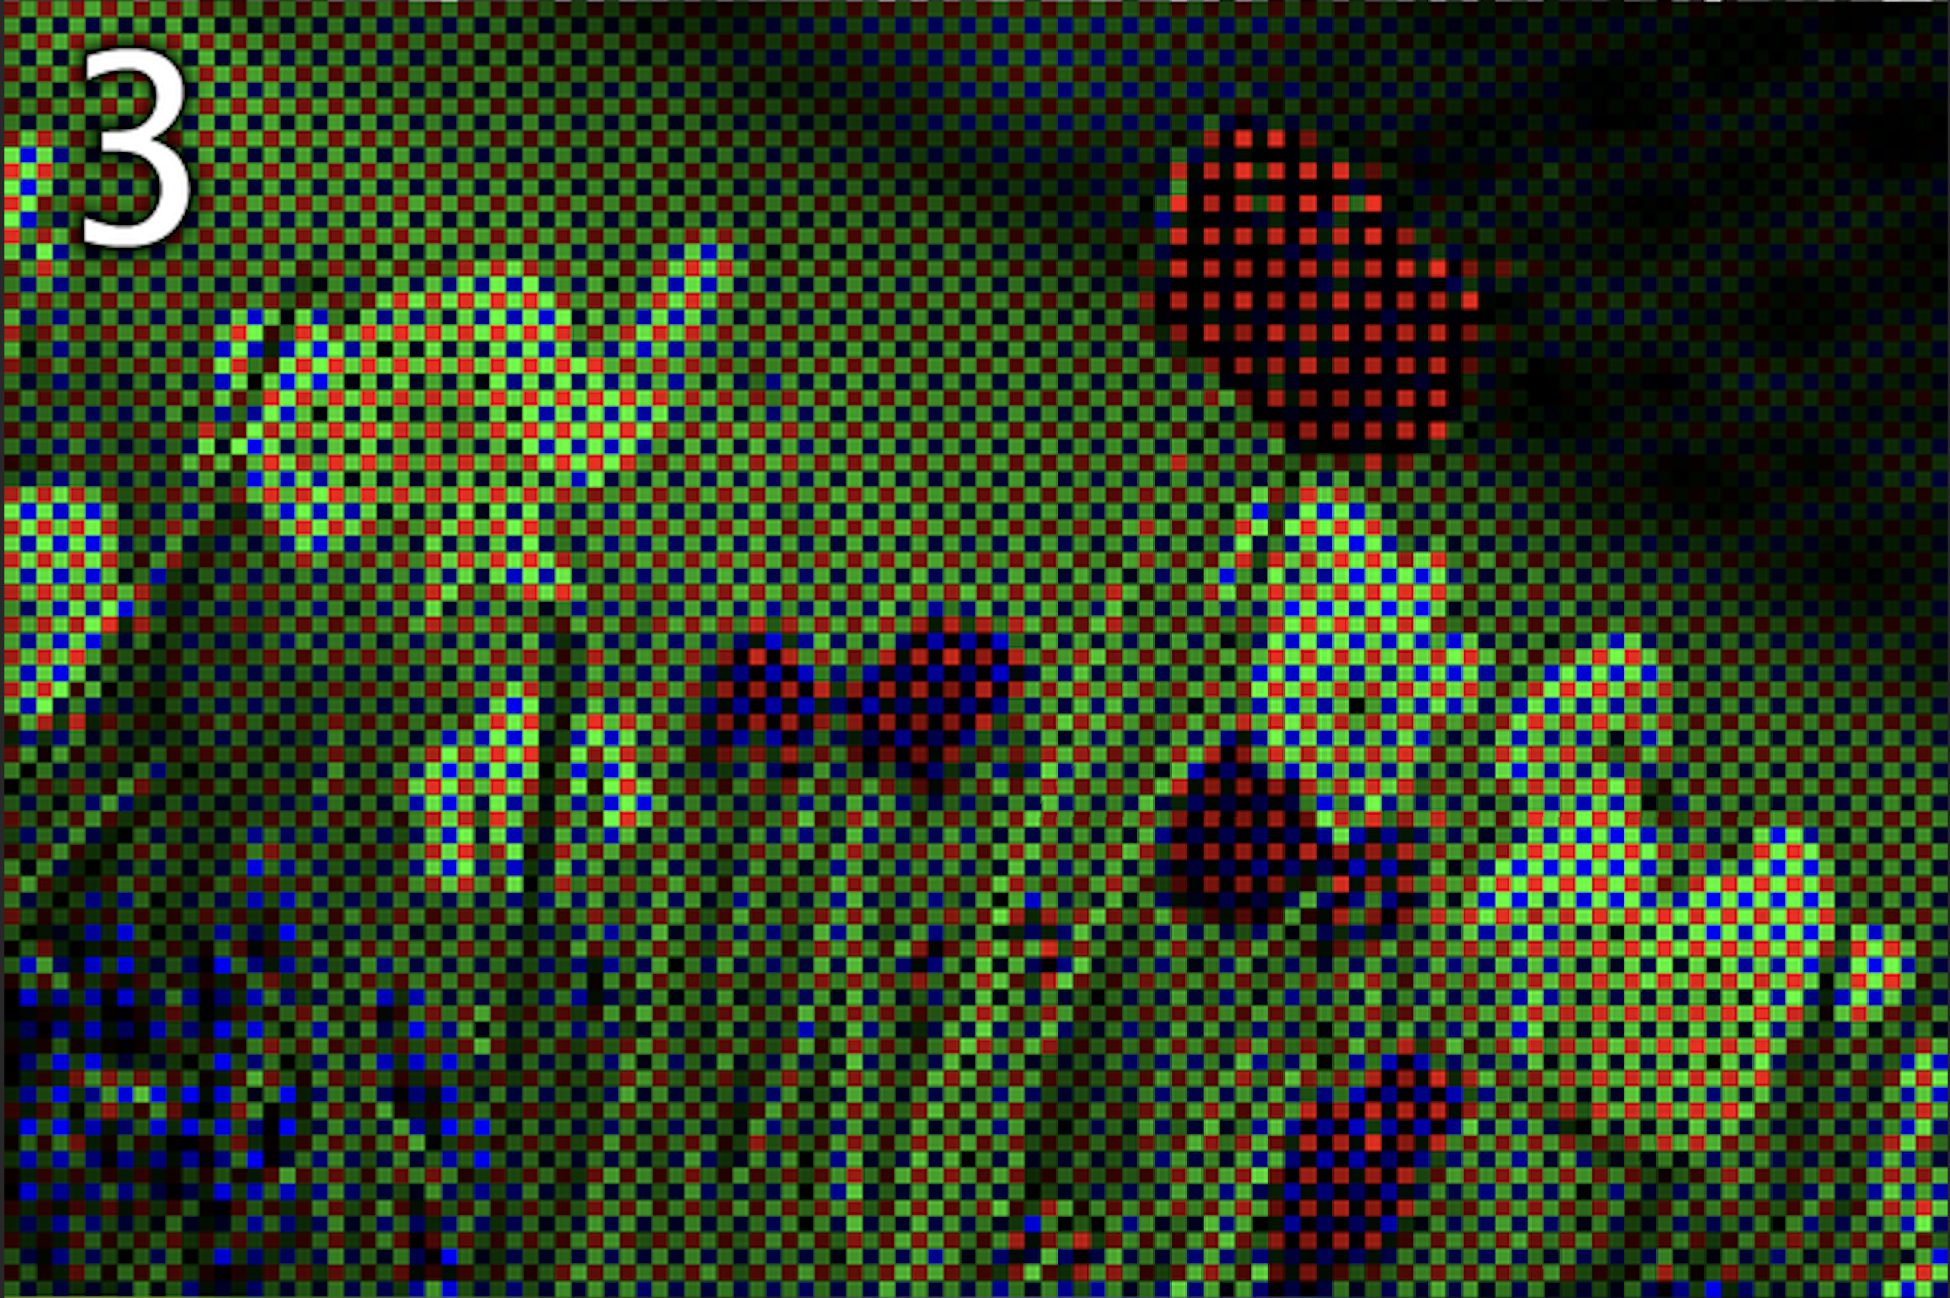
\includegraphics[width=0.5\textwidth]{./figures/bayer-3.png}
		\end{center}
		\caption{Output color-coded with Bayer filter colors.}
	\end{figure}
\end{frame}

\begin{frame}
	\begin{figure}
		\begin{center}
			\includegraphics[width=0.5\textwidth]{./figures/bayer-4.png}
		\end{center}
		\caption{Reconstructed image after interpolating missing color information.}
	\end{figure}
\end{frame}

\begin{frame}
	\begin{figure}
		\begin{center}
			\includegraphics[width=0.5\textwidth]{./figures/filter-wheel-MIRI.jpg}
		\end{center}
		\caption{The usage of filter wheel to record different wavelength.}
	\end{figure}
\end{frame}
% --- Conclusion --- %
\section{References \& Conclusion}

\begin{frame}{References}
	\bibliographystyle{plain}
	\bibliography{references}
\end{frame}

% ---- The End ---- %
\begin{titleframe}{Thank you for listening!}
\end{titleframe}

\end{document}
